%% LyX 2.1.4 created this file.  For more info, see http://www.lyx.org/.
%% Do not edit unless you really know what you are doing.
\documentclass[english]{article}
\usepackage[T1]{fontenc}
\usepackage[latin9]{inputenc}
\usepackage{geometry}
\geometry{verbose,tmargin=2cm,bmargin=2cm,lmargin=2cm,rmargin=2cm}
\usepackage{float}
\usepackage{units}
\usepackage{amsmath}
\usepackage{amsthm}
\usepackage{graphicx}

\makeatletter
%%%%%%%%%%%%%%%%%%%%%%%%%%%%%% User specified LaTeX commands.
\usepackage{tikz}
\usetikzlibrary{shapes,arrows}
\usepackage{tocloft}

\makeatother

\usepackage{babel}
\begin{document}

\title{ENGN6528 - Computer Vision: Term Project}


\author{John Aslanides}
\maketitle
\begin{abstract}
We present a simple license plate recognition system which uses morphology-based
segmentation, and artificial neural network-based recognition. The
system achieves a license plate recognition rate of 75\% on typical
cropped Australian license plate images. We propose several methods
to improve the classification rate.
\end{abstract}
\global\long\def\b#1{\boldsymbol{#1}}



\section{Introduction}

Automated license plate recognition is an important application of
computer vision that is useful in numerous settings, including traffic
data collection, law enforcement, motorway toll collection, and managing
parking lots \cite{Nijhuis-95}. A system with the capability to robustly
and accurately recognise license plates from various jurisdictions
can be of great value when applyed to any of the above tasks; for
this reason there has been significant research and development in
this area in the past two decades \cite{Bailmare-13}. The most typical
license plate recognition system involves three steps \cite{Ozturk-2012}: 
\begin{enumerate}
\item localising a license plate within a cluttered scene, possibly containing
more than one car,
\item segmenting the license plate into its constituent glyphs, and 
\item performing optical character recognition (OCR) on these glyphs to
obtain the license plate string. 
\end{enumerate}
The problem we will be solving with our system consists of steps (2)
and (3); that is, the images we will be dealing with consist of cropped
license plates, and the task is to output a string corresponding to
the correct license plate.


\section{Background}

There has been considerable ongoing research in the area of license
plate recognition over the last twenty years, with a rich literature
exploring different ideas and techniques. Below we provide some background
on these techniques, concentrating on segmentation and recognition
(we assume that license plate localisation and rectification has already
been performed). We also provide a brief review of the theory of neural
networks.


\subsection{License Plate Segmentation}

There are many difficulties in license plate character segmentation.
Some of these include: image noise, plate frame occlusion, presence
of bolts or rivets, and extraneous slogans and images on the license
plate. There are numerous approaches to dealing with these in the
literature; these include segmentation based on the Hough transform
\cite{Zhang-03}, projection histograms \cite{Hegt-98}, clustering
\cite{Zheng-2011}, template matching \cite{Pan-2008}, and morphology
\cite{Karthikeyan-13}. The choice of segmentation technique seems
to be largely a matter of taste; no single technique explored in the
literature dominates the others in terms of performance; in one review
study that compared numerous techniques, a variation in performance
of less than 5\% was recorded \cite{Karthikeyan-13}. For this reason,
there is no true `state of the art' method, just a collection of different
techniques with their own advantages and disadvantages. 

\begin{figure}[h]
\begin{centering}
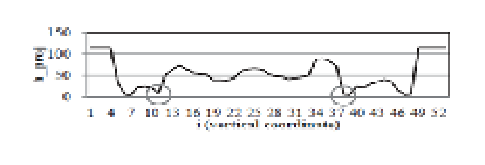
\includegraphics{Figures/hor_proj}
\par\end{centering}

\begin{centering}
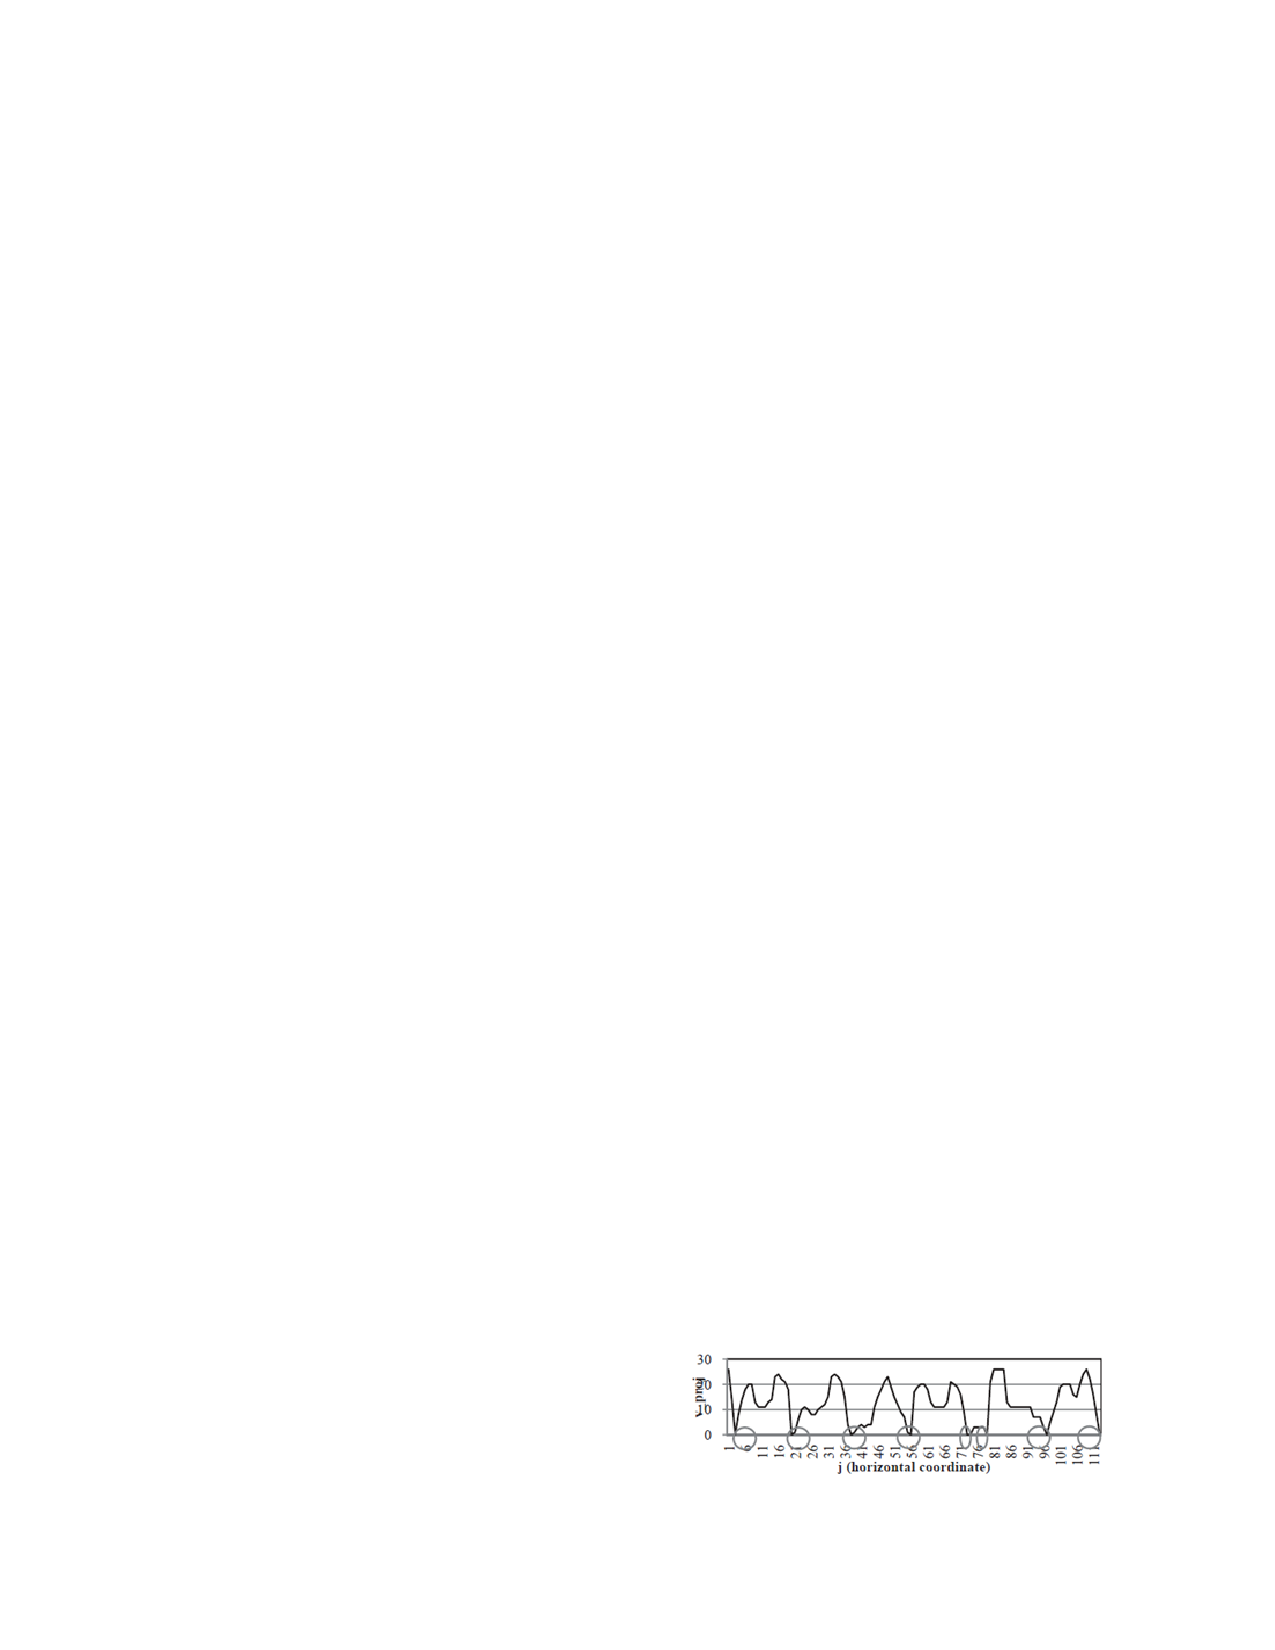
\includegraphics{Figures/vert-proj}
\par\end{centering}

\caption{An example of the projection histogram technique. Troughs in the histogram
correspond to gaps between symbols \cite{Karthikeyan-13}.}
\end{figure}



\subsection{License Plate Recognition}

Once the license plate characters have been segmented, the problem
essentially reduces to the standard OCR problem: given an image of
a character represented in the pixel domain, to recognise the character.
Again, there are numerous approaches to this problem in the license
plate context; these include `classical' methods such as template
matching and the Hotelling transform \cite{Hegt-98}, and learning
based methods such as support vector machines (SVM) and neural networks
\cite{akoum-2009,bhushan-2013,carrera-2009,ZhengHao-2014}. 


\subsection{Artificial Neural Networks}

Artificial neural networks (ANNs) are a powerful tool for classification
and function approximation, which have been effective in many diverse
domains and settings\footnote{For an interesting overview of recurrent neural networks and their
uses, see `The Unreasonable Effectiveness of Recurrent Neural Networks'
at http://karpathy.github.io/2015/05/21/rnn-effectiveness/.}. Algorithms that employ neural networks are the state of the art
in many domains, including handwriting and character recognition \cite{lecun-98}.
The setup of a feed-forward neural network is as follows. The network
is composed of layers of `neurons', which each take as input a linear
combination of the outputs of the previous layer, and apply a nonlinear
activation function to this input:
\[
a_{j}^{\left(i\right)}=\sigma\left(\sum_{k=1}^{N_{i-1}}w_{ij}^{\left(i-1\right)}a_{k}^{\left(i-1\right)}\right).
\]


Here we define $a_{j}^{\left(i\right)}$ as the output of neuron $j$
in layer $i$, the $w_{ij}^{\left(i-1\right)}$ are the weights joining
layers $i-1$ and $i$, and $\sigma$ is the nonlinear activation
function, which is typically the logistic sigmoid:
\[
\sigma\left(x\right)=\frac{1}{1+e^{-x}}.
\]


Note that in the typical setup, each layer is fully connected to its
adjacent layers. The first layer is the input data, and the last layer
is the output (corresponding to a class, or regression, depending
on the setting). Intermediate layers are called `hidden layers', and
these can be thought of as learning intermediate basis functions or
representations for the data. Considered layer-by-layer, a neural
network comprises an iterated series of generalised linear models.
The entire $L$-layer network can be written down as a vector-valued
function with elements given by
\[
y_{i}\left(\b x\right)=\sigma\left(\sum_{i_{L-1}=1}^{N_{L-1}}w_{ii_{L-1}}^{\left(L-1\right)}\sigma\left(\sum_{i_{L-2}=1}^{N_{L-2}}w_{i_{L-1}i_{L-2}}^{\left(L-2\right)}\sigma\left(\dots\sigma\left(\sum_{i_{1}=1}^{N_{1}}w_{i_{2}i_{1}}^{\left(1\right)}x_{i_{1}}\right)\right)\right)\right),
\]


where $w_{ij}\left(k\right)$ is the weight between unit $i$ of layer
$k-1$ and unit $j$ of layer $k$.

The classifier itself will simply take the index of the maximum value
of $\b y$; this is interpreted as the class that the input $\b x$
belongs to, with highest probability, according to the model implied
by the network. Hence out classifier $C$ simply takes the output
of the neural network and computes the $\arg\max$:
\[
C\left(\b x\right)=\arg\max_{i}y_{i}\left(\b x\right).
\]
Training can then be done in conjunction with gradient descent and
an appropriate loss function $E$ using the backpropagation algorithm,
which amounts to an application of the chain rule for derivatives
\cite{bishop-06}: 
\[
\frac{\partial E}{\partial w_{ij}^{\left(l-1\right)}}=\frac{\partial a_{j}^{\left(l-1\right)}}{\partial w_{ij}^{\left(l-1\right)}}\sigma'\left(a_{j}^{\left(l\right)}\right)\sum_{k}w_{kj}^{\left(l\right)}\frac{\partial E}{\partial a_{k}^{\left(l\right)}}.
\]


It is important to note that the neural network has many discrete
symmetries: there are a large number of permutations of the weights
which leave the network invariant. This means that the objective function
$E$ is non-convex, and optimization via gradient descent methods
is not guaranteed to find the global minimum. This is a limitation
of neural networks when compared with SVMs, since the optimization
involved in SVM is a quadratic program, and is therefore convex \cite{cortes-95}. 

\begin{figure}
\begin{centering}
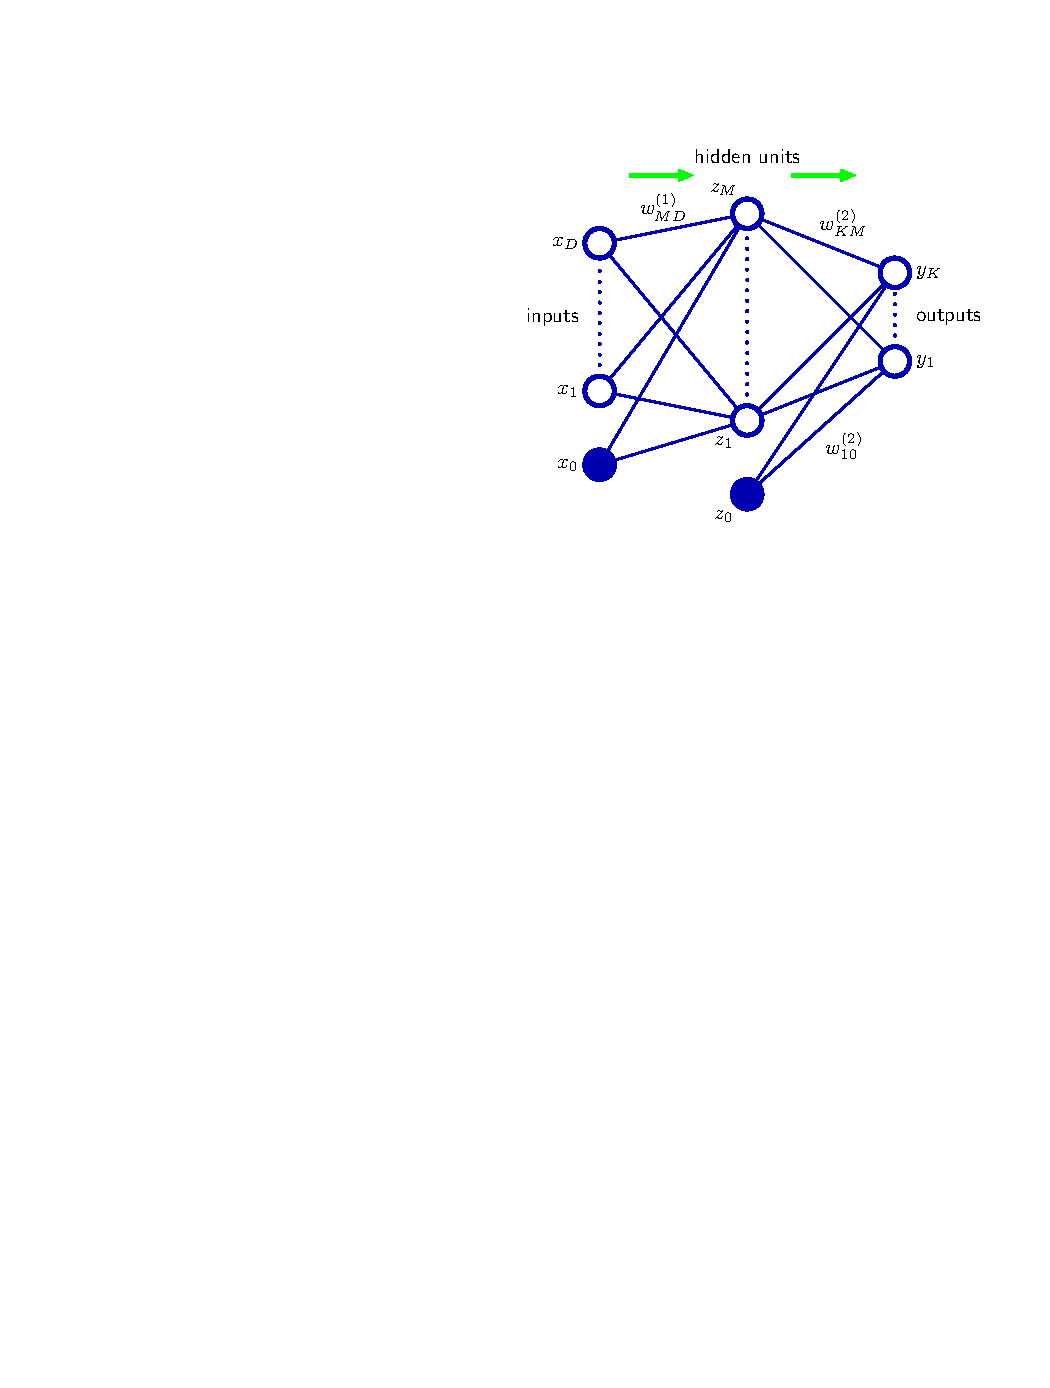
\includegraphics{Figures/neuralnet_cartoon}
\par\end{centering}

\caption{Architecture of a fully connected single hidden-layer feedforward
neural network. The filled nodes $x_{0}$ and $z_{0}$ are bias terms. }


\end{figure}



\section{Design approach}


\subsection{License Plate Segmentation}

We first take the RGB input image and convert it to greyscale by extracting
only the green channel. We initially crop the edges\footnote{We find empirically that cropping $10\%$ from the top and bottom,
and $3\%$ from the sides is effective.}, since we can be sure they don't contain any important information,
and they typically present a large connected component (the plate
border) which we want to be rid of for the following image analysis.
We then binarize the resulting image, determining the threshold through
Otsu's method\footnote{http://en.wikipedia.org/wiki/Otsu\%27s\_method.}.
We use a morphology-based approach. The general idea is to take advantage
of the fact that we know \emph{a priori }that the glyphs we are interested
in will have certain properties:
\begin{itemize}
\item they collectively take up a significant portion of the license plate
area,
\item their upper and lower edges are colinear, and
\item their aspect ratio is less than $1$; that is, glyphs are taller than
they are wide.
\end{itemize}
Using this knowledge, our segmentation algorithm uses a sequence of
simple morphological operations to first generate `candidate' cropped
regions of the license plate, attempt to clean them up of extraneous
details (such as bolts and rivets), and test them to see whether they
fulfil the above requirements\footnote{The MATLab function is found in ${\tt Code\backslash image\_partition.m}$.}.
If a suitable number of candidates makes it through the testing process,
we've succeeded, and we return the segmentation. If not, we try again,
recursively calling the partition algorithm, by first inverting the
colors of the plate, and then by progressively cropping the plate
down, if we still don't find any candidate regions. 

To generate the candidate regions, we initially take a similar approach
to that used in the C-Lab1 morphology exercise, in which the goal
is to segment lines of text from a textbook. We dilate the image horizontally
by a wide structuring element, and crop the image to the vertical
dimensions of the largest connected component that results. We then
dilate vertically with a tall structuring element, and use connected
component analysis\footnote{We use MatLab's implementation ${\tt bwconncomp}$, which uses the
flood fill algorithm: http://en.wikipedia.org/wiki/Flood\_fill.} on the result to segment the image into several candidate images.
Typical plates will have between 10-20 candidates generated by this
process. The vast majority are spurious candidates, and we eliminate
them with numerous tests that follow.

Once we have a suitable number of candidate image regions, we progressively
narrow them down by applying several tests to them. Let $\mathcal{C}=\left\{ C_{i}\right\} _{i=1}^{N}$
be the set of candidates, and let $H\left(C_{i}\right)$ and $W\left(C_{i}\right)$
be the height and width of candidate region $C_{i}$ respectively.
Then for each candidate $C_{i}$ we prune it from the list if it fails
any of the following tests:
\begin{enumerate}
\item Is the aspect ratio $R$
\[
R\left(C_{i}\right)=\frac{H\left(C_{i}\right)}{W\left(C_{i}\right)}
\]



within the interval $[1,10]$?


We choose a lower bound of $1$ by the empirical observation that
all glyphs in Australian license plates appear to be taller than they
are wide. The upper bound of $10$ is purely to accomodate the glyphs
`$1$' and `$I$'; all other glyphs have aspect ratios roughly in
the interval $\left[1,2\right]$. This criterion is quite useful for
trimming out parts of slogans or other artifacts of the morphological
segmentation, since these often have aspect ratios outside this interval.

\item Is the mean intensity\footnote{Recall that these are binary images, so we are just counting the proportion
of white pixels in the candidate region.} 
\[
\bar{I}\left(C_{i}\right)=\frac{\sum_{j=1}^{H\left(C_{i}\right)}\sum_{k=1}^{W\left(C_{i}\right)}\left[C_{i}\right]_{jk}}{H\left(C_{i}\right)W\left(C_{i}\right)}
\]



in the interval $\left[0.1,0.9\right]$?


Again, we find empirically that this is a useful heuristic for removing
non-glyph segments. For example, the `hyphen-like' separator often
found between the first three and last three digits of the license
plate is excluded by this test, since it is almost completely white. 

\item Is the candidate's height within $10\%$ of the mode of all passing
candidates?
\[
\frac{H\left(C_{i}\right)-{\tt mode}\left(\mathcal{H}\right)}{{\tt mode}\left(\mathcal{H}\right)}<0.1,
\]



where $\mathcal{H}=\left\{ H\left(C_{i}\right)\ |\ C_{i}\in\mathcal{C},\ C_{i}\ \text{passing}\right\} $
is the set of heights of passing candidates. 


This condition is quite stringent, and takes advantage of our prior
knowledge that all the glyphs must be approximately the same height.
It gets rid of plausible-looking candidate regions which contain,
for example, state logos or other symbols or imagery. 

\end{enumerate}
The whole segmentation pipeline is laid out in Figure \ref{fig-pipeline},
with accompanying plate images to illustrate. 

\begin{figure}[h]
\begin{centering}
\usetikzlibrary{positioning}
\tikzstyle{block} = [rectangle, draw, fill=blue!20, text width=10em, text centered, rounded corners, minimum height=3em] 
\tikzstyle{newblock} = [rectangle, draw, fill=blue!20, node distance=5cm, text width=10em, text centered, rounded corners, minimum height=3em] 
\tikzstyle{choice} = [diamond, draw, fill = blue!20, node distance=2cm, text width=4em, text centered]
\tikzstyle{line} = [draw, -latex'] 
\tikzstyle{imgblock} = [draw, rectangle, node distance=2cm, minimum height=2em,rounded corners]

\begin{tikzpicture}[node distance = 2cm, auto]

    \node [block] (threshold) {threshold and binarize};
    \node [block, below of=threshold] (dilate) {dilate};
    \node [block, below of=dilate] (candidates) {candidate regions};
    \node [block, below of=candidates] (filter) {filter candidates};
	\node [choice, below of=filter, aspect=2] (decision) {$|\mathcal{C}|>2$?};
	\node [block, below of=decision] (neural) {neural network};
	\node [newblock, right of = decision] (flip) {invert colors};
	\node [block, below of=neural] (string) {output string};
	
    \path [line] (threshold) -- (dilate);
    \path [line] (dilate) -- (candidates);
    \path [line] (candidates) -- (filter);
	\path [line] (filter) -- (decision);
	\path [line] (decision) -- node [near start] {No} +(3,0) coordinate (my coord) -- (flip.west);
    \path [line] (decision.south) -- node {Yes}  +(0,-20pt)  --  (neural);
	\path [line] (flip.north) |- (threshold);
	\path [line] (neural) -- (string);


	\node [imgblock, left=4cm of threshold] (cropimg) {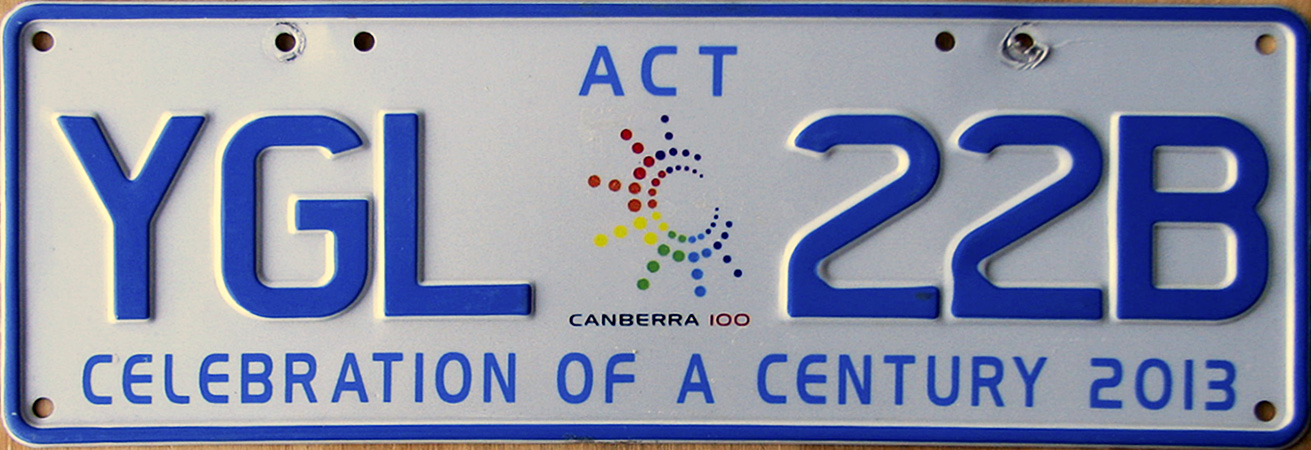
\includegraphics[height=3em,width=8em]{partitioning/img.jpg}};
	\node [imgblock, left=4cm of dilate] (hor_dilate) {
\includegraphics[height=3em, width=8em]{partitioning/hor_dilate.png}};
	\node [imgblock, left=4cm of candidates] (vert_dilate) {
\includegraphics[height=3em, width=8em]{partitioning/vert_dilate.png}};
	\node [imgblock, left=4cm of filter] (candidates) {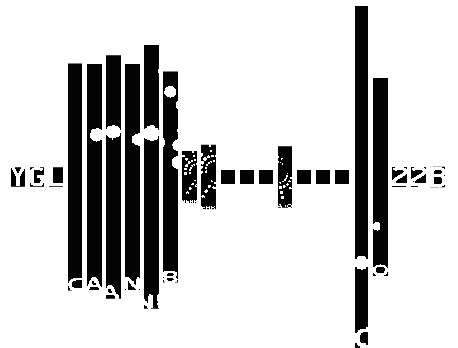
\includegraphics[height=3em, width=8em]{partitioning/candidates.png}};
	\node [imgblock, left=4.5cm of decision] (output) {
\includegraphics[height=3em, width=8em]{partitioning/output.png}};
	\node [rectangle, draw, fill=white!20, text width=8em, text centered, rounded corners, minimum height=3em, left=4cm of string] (strout) {YGL22B};
	
	\path [line] (cropimg) -- (hor_dilate);
	\path [line] (hor_dilate) -- (vert_dilate);
	\path [line] (vert_dilate) -- (candidates);
	\path [line] (candidates) -- (output);
	\path [line] (output) -- (strout);

\end{tikzpicture}
\par\end{centering}

\label{fig-pipeline}

\caption{\textbf{Right: }License plate recognition pipeline. \textbf{Left:
}Example of the morphological segmentation process.}
\end{figure}



\subsection{Neural Network training}

We train a single hidden layer neural network on a dataset of over
36,000 images of computer fonts, taken from the Chars74K dataset\footnote{This can be found at http://www.ee.surrey.ac.uk/CVSSP/demos/chars74k/.}.
We take as inputs $32\times32$ pixel square binary images, which
correspond to input vectors of length $1024$; The neural network
architecture used is illustrated in Figure \ref{fig-nn-architecture}.
We experimented with different feature representations, including
integral representations such as the Radon transform\footnote{http://en.wikipedia.org/wiki/Radon\_transform.},
but found little to no improvement in performance. We use the 1-of-$K$
encoding to represent our output vectors, which has $36$ classes
($26$ alphabetical, and $10$ numerical glyphs). We also use the
cross entropy loss function
\[
E\left(y,t\right)=-t\log y-(1-t)\log(1-y).
\]


We use an $l_{2}$ regularizer on the weights, and let MATLab randomly
divide the training set into training, test, and validation sets to
avoid overfitting. We train for 76 iterations of scaled conjugate
gradient descent\footnote{http://en.wikipedia.org/wiki/Conjugate\_gradient\_method.},
which takes 7 minutes on a 2.3 GHz i5 Macbook Pro with 16GB of memory.
The mean cross-entropy error on the training set with the learned
weights is $10^{-3}$.

\begin{figure}
\begin{centering}
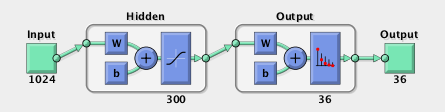
\includegraphics{Figures/neuralnet}
\par\end{centering}

\label{fig-nn-architecture}

\caption{Architecture of our feedforward neural network.}


\end{figure}



\section{Implementation and experimental results}

The system is implemented with MATLab scripts and functions, which
we include in the ${\tt Code}$ directory. The main segmentation work
is done by ${\tt image\_partition}$, with calls to a helper function
${\tt tallestcomponent}$. The neural network is trained beforehand,
and is stored in a ${\tt .mat}$ file for ease of retrieval and re-use.
The ${\tt classify}$ function performs the license plate segmentation
and recognition. See Appendix \ref{sec:How-to-run} for details on
how to run the system. 

We tested the system on 70 cropped Australian license plate images
taken from Wikipedia\footnote{http://en.wikipedia.org/wiki/Vehicle\_registration\_plates\_of\_Australia.}
and Plateshack\footnote{http://www.plateshack.com/y2k/.}. Some sample
plates with their segmentations are shown in Figure \ref{fig-samples}.
On this test dataset, we achieved $94.9\%$ glyph recognition accuracy,
and $74.3\%$ overall plate accuracy\footnote{Note that we take ``O'' to be equivalent to ``0'', and ``1''
to be equivalent to ``I''. This is common prctice, as in many US
states, authorities do not distinguish between these glyphs.}. Note that the system makes no distinction between plates from different
states; the same algorithm is used for segmentation and recognition
for all license plates.

\begin{figure}[H]
\begin{centering}
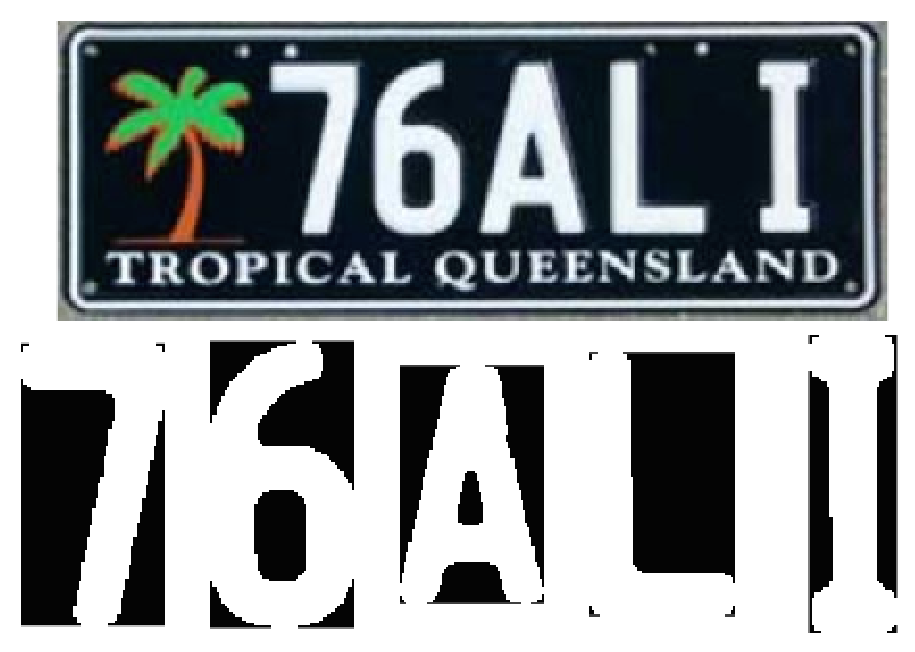
\includegraphics[scale=0.5]{Figures/76ALI}$\qquad$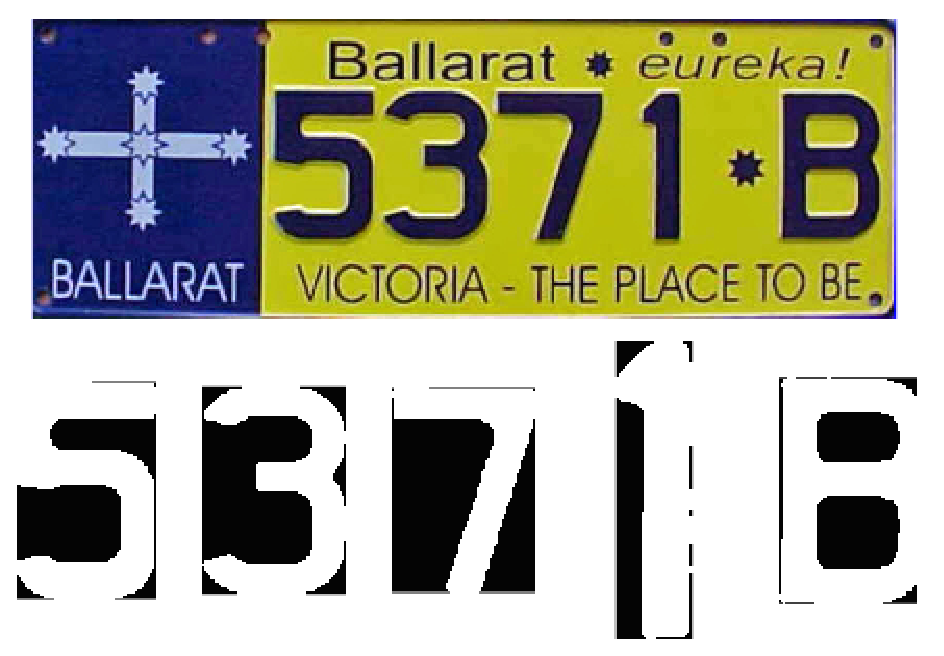
\includegraphics[scale=0.5]{Figures/5371B}
\par\end{centering}

\quad{}\quad{}\quad{}\quad{}\quad{}\quad{}\quad{}\quad{}\quad{}\quad{}\quad{}\quad{}\quad{}(a)\quad{}\quad{}\quad{}\quad{}\quad{}\quad{}\quad{}\quad{}\quad{}\quad{}\quad{}\quad{}\quad{}\quad{}\quad{}\quad{}\quad{}\quad{}\quad{}\quad{}\quad{}\quad{}(b)

\begin{centering}
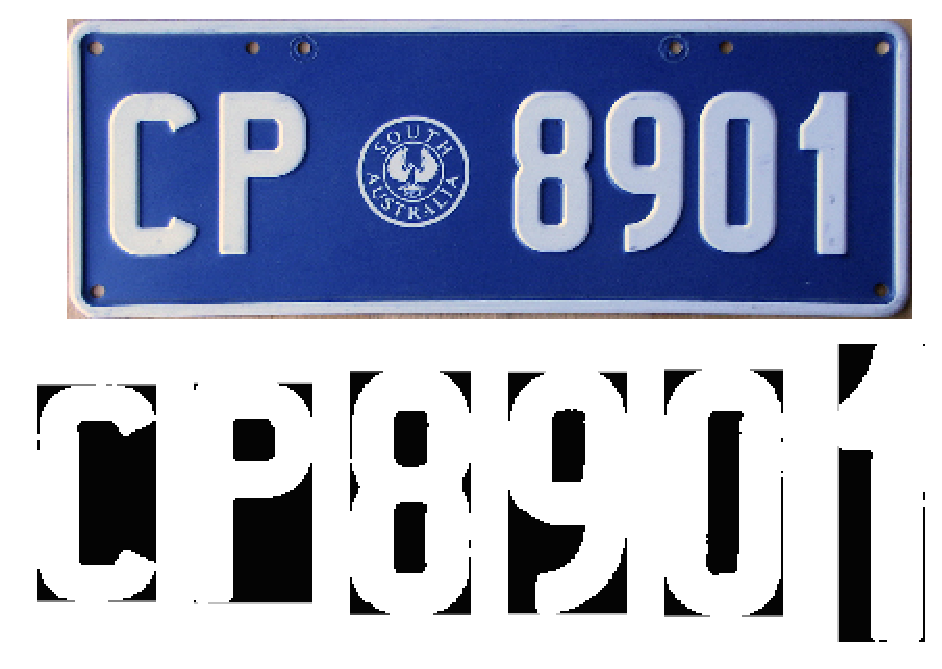
\includegraphics[width=7cm,height=3.5cm]{Figures/CP8901}$\qquad$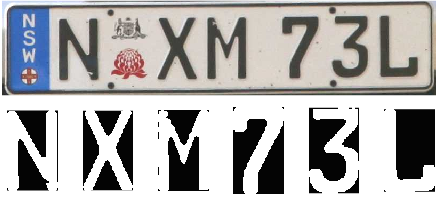
\includegraphics[scale=0.5]{Figures/NXM73L}
\par\end{centering}

\quad{}\quad{}\quad{}\quad{}\quad{}\quad{}\quad{}\quad{}\quad{}\quad{}\quad{}\quad{}\quad{}(c)\quad{}\quad{}\quad{}\quad{}\quad{}\quad{}\quad{}\quad{}\quad{}\quad{}\quad{}\quad{}\quad{}\quad{}\quad{}\quad{}\quad{}\quad{}\quad{}\quad{}\quad{}\quad{}(d)

\begin{centering}
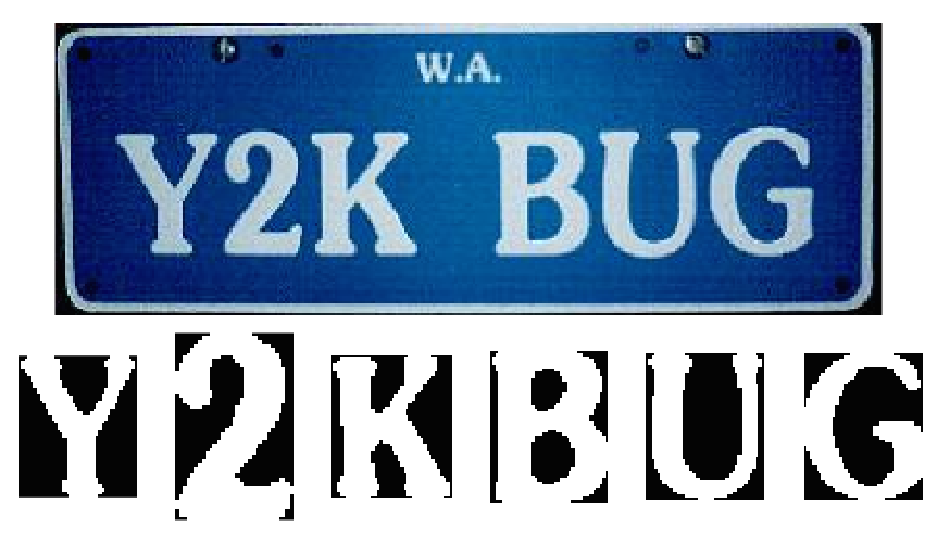
\includegraphics[scale=0.5]{Figures/Y2KBUG}$\qquad$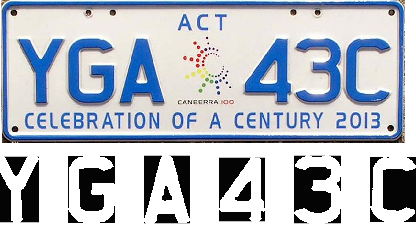
\includegraphics[scale=0.5]{Figures/YGA43C}
\par\end{centering}

\quad{}\quad{}\quad{}\quad{}\quad{}\quad{}\quad{}\quad{}\quad{}\quad{}\quad{}\quad{}\quad{}(e)\quad{}\quad{}\quad{}\quad{}\quad{}\quad{}\quad{}\quad{}\quad{}\quad{}\quad{}\quad{}\quad{}\quad{}\quad{}\quad{}\quad{}\quad{}\quad{}\quad{}\quad{}\quad{}(f)

\label{fig-samples}

\caption{Six license plate examples, accompanied by their segmentations. Note
that these plates present numerous challenges, including: large non-glyph
graphics in \textbf{(a) }and \textbf{(b)}; uneven lighting and contrast
in \textbf{(e)}; unusual glyph spacing in \textbf{(d)}. Note also
the varying background and foreground colours, and the varying fonts
used. These plates are all correctly segmented and recognised by the
system.}
\end{figure}



\section{Conclusions}

Below we discuss the performance of the system, and propose numerous
improvements. We also outline some of the learning outcomes from the
project.


\subsection{Limitations and possible extensions}

The system has two main limitations: the plate segmentation algorithm
assumes that we are already given a cropped license plate image. Adding
a plate localization routine could address this issue, but it is outside
the scope of the project. We'll focus on our attention on the second
issue, which relates to the performance of the neural network.

The single-glyph recognition rate of $94.9\%$ achieved by the neural
network is reasonably high, but compounding this over a mean plate
length of six glyphs yields around the $75\%$ plate accuracy that
we achieved. If we require a $95\%$ plate recognition accuracy, this
requires an accuracy of $0.95^{\nicefrac{1}{6}}\approx99\%$ glyph
accuracy. To achieve this level of accuracy in the neural network,
there are a few possible approaches:
\begin{itemize}
\item Train the neural network on labelled license plates. This has the
advantage of showing the neural network examples of the fonts used
in the license plates, including the noise associated with the images.
This should address the issue we see in Figure \ref{sb77hw}(a). The
disadvantage is that this would require a large database of labelled
Australian license plates images, which is not easily available, to
the author's knowledge.
\item Use more advanced features such as line/loop feature detectors used
in Cuneiform and Tesseract\cite{smith-07}, or using SIFT \cite{Kae-09}.
We could augment the pixel representation with other global features,
such as topological invariants\footnote{http://en.wikipedia.org/wiki/Topological\_property.},
or other characteristics. Feature engineering such as this would probably
help to disambiguate similar characters such as 'G' and '6', which
are commonly misclassified by my system (see Figure \ref{sb77hw}(b)).
\item Use a state-of-the-art Convolutional Neural Network classifier, or
a boosted classifier\footnote{Using an algorithm such as AdaBoost.}.
\end{itemize}
\begin{figure}
\begin{centering}
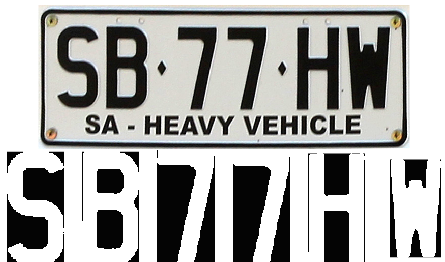
\includegraphics[scale=0.5]{Figures/SB77HW}$\quad$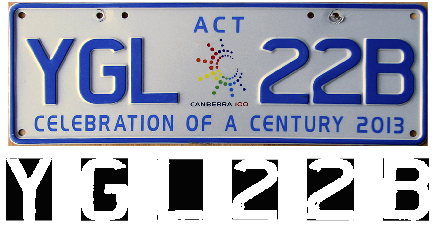
\includegraphics[scale=0.5]{Figures/YGL22B}
\par\end{centering}

\label{sb77hw}

\caption{\textbf{Left: }The input plate is `SB77HW', but the system classifies
it as as `SB77HN'. This is symptomatic of the difficulties presented
by the unusual, compressed fonts used in license plates. \textbf{Right:
}The input plate is clearly `YGL22B', but the system classifies it
as 'Y6L22B'. This misclassification could possibly be improved by
including extra features such as closed loop detectors, or computing
how many disconnected regions there are.}
\end{figure}



\subsection{Learning outcomes}

In the process of doing this project, I learned a number of things:
\begin{itemize}
\item I discovered and evaluated different solutions to the license plate
recognition problem by performing a review of the international computer
vision literature. 
\item I followed test-driven engineering principles, by implementing a test
harness for the system, and subsequently making incremental changes
to the system in an attempt to improve the test results.
\item I trained a neural network on a large dataset and explored different
feature representations.
\item I experimented with numerous image processing techniques and became
familiar with their implementations and uses.
\end{itemize}
\appendix

\section{How to run the Matlab code\label{sec:How-to-run}}

The code is stored in the ${\tt Code}$ directory; this directory
will have to be added to your MATLab path. The main top level method
is ${\tt classify}$, which takes as inputs a neural net, and an RGB
image. A neural net is saved in ${\tt Data/net.mat}$. Load this into
the main namespace with ${\tt load('Data/net.mat')}$. Then, you can
call ${\tt classify(im,net)}$, where ${\tt im}$ is a $M\times N\times3$
array of unsigned $8$-bit integers, of the kind returned by ${\tt imread}.$
Alternatively, you can  call the ${\tt demo()}$ function which will
automatically run through the 70 plates included, showing the original,
the segmentation, and printing the recognised output to the MATLab
console. 

\bibliographystyle{unsrt}
\bibliography{bib}

\end{document}
